\begin{figure}
\centering
\begin{subfigure}{0.45\textwidth}
\includemedia[width=\textwidth,activate=onclick,addresource=images/animations/ukf.mp4,flashvars={source=images/animations/ukf.mp4&autoPlay=true&loop=true}]{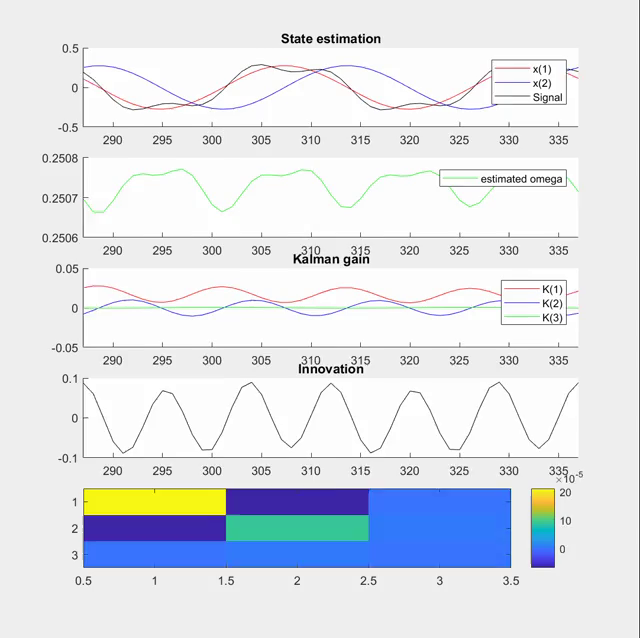
\includegraphics[width=\textwidth]{images/animations/ukf.png}}{VPlayer.swf}
\caption{Signal, estimation, Kalman gain and covariance matrix P\footnotemark.
$\omega_{\text{true}} = 0.25076 \ \sfrac{\text{rad}}{\text{sample}}$ (1760 \si{\hertz})}
\label{fig:ukf_estimation}
\end{subfigure}
\quad
\begin{subfigure}{0.4\textwidth}
\includemedia[width=\textwidth,activate=onclick,addresource=images/animations/sp.mp4,flashvars={source=images/animations/sp.mp4&autoPlay=true&loop=true}]{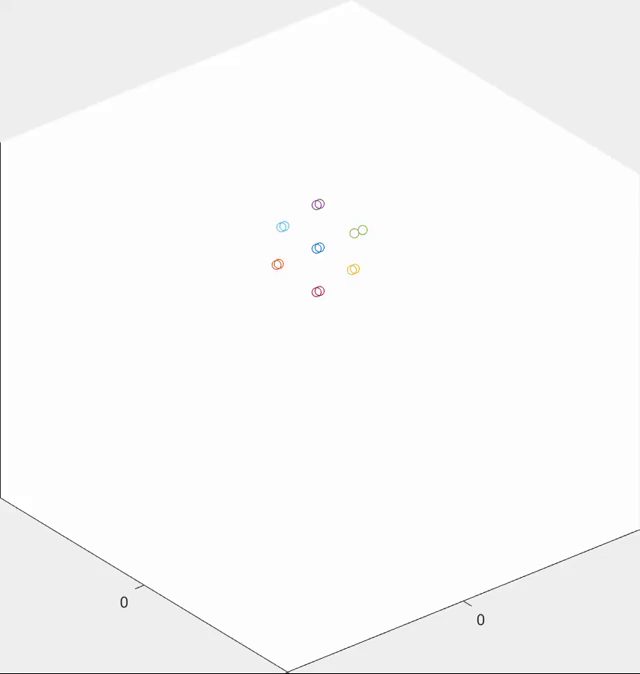
\includegraphics[width=\textwidth]{images/animations/sp.png}}{VPlayer.swf}
\caption{Evolution of sigma points in the state space}
\label{fig:ukf_sigmapoints}
\end{subfigure}

\caption{UKF visualizations}
\label{fig:ukf_visualizations}
\end{figure}
\footnotetext{It is interesting to notice how the absolute values of the elements of P are proportional to the slope of the component in the figure: higher rate of change means higher estimation variance.}